% **************************************************
% Document Class Definition
% **************************************************
\documentclass[%
	paper=A4,					% paper size --> A4 is default in Germany
	twoside=false,				% onesite or twoside printing
	openright,					% doublepage cleaning ends up right side
	parskip=full,				% spacing value / method for paragraphs
	chapterprefix=true,			% prefix for chapter marks
	11pt,						% font size
	headings=normal,			% size of headings
	bibliography=totoc,			% include bib in toc
	listof=totoc,				% include listof entries in toc
	titlepage=on,				% own page for each title page
	captions=tableabove,		% display table captions above the float env
	draft=false,				% value for draft version
]{scrreprt}%

\usepackage[utf8]{inputenc}		% defines file's character encoding

% **************************************************
% Debug LaTeX Information
% **************************************************
%\listfiles

% **************************************************
% Information and Commands for Reuse
% **************************************************
\newcommand{\thesisTitle}{CS807 - Final Project}
\newcommand{\thesisName}{André E. dos Santos \\ Jhonatan S. Oliveira}
\newcommand{\thesisSubject}{Resource Constrained Computing}
\newcommand{\thesisDate}{March, 2016}
\newcommand{\thesisVersion}{Final Version}

\newcommand{\thesisFirstReviewer}{Dr. David Gerhard}
\newcommand{\thesisFirstReviewerUniversity}{\protect{University of Regina}}
\newcommand{\thesisFirstReviewerDepartment}{Department of Computer Science}

\newcommand{\thesisSecondReviewer}{Mr. Trevor Tomesh}
\newcommand{\thesisSecondReviewerUniversity}{\protect{University of Regina}}
\newcommand{\thesisSecondReviewerDepartment}{Department of Computer Science}

\newcommand{\thesisFirstSupervisor}{Dr. David Gerhard}
\newcommand{\thesisSecondSupervisor}{Mr. Trevor Tomesh}

\newcommand{\thesisUniversity}{\protect{University of Regina}}
\newcommand{\thesisUniversityDepartment}{Department of Computer Science}
\newcommand{\thesisUniversityInstitute}{N/A}
\newcommand{\thesisUniversityGroup}{N/A 2}
\newcommand{\thesisUniversityCity}{Regina}
\newcommand{\thesisUniversityStreetAddress}{3737 Wascana Pkwy}
\newcommand{\thesisUniversityPostalCode}{S4S 0A2}

% **************************************************
% Load and Configure Packages
% **************************************************
\usepackage[utf8]{inputenc}		% defines file's character encoding
\usepackage[english]{babel} % babel system, adjust the language of the content
\usepackage{marginnote} %margin note
\usepackage{paralist} %inline list
\usepackage{hyperref}
\usepackage[					% clean thesis style
	figuresep=colon,%
	sansserif=false,%
	hangfigurecaption=false,%
	hangsection=true,%
	hangsubsection=true,%
	colorize=full,%
	colortheme=bluemagenta,%
	bibsys=bibtex,
]{cleanthesis}

\hypersetup{					% setup the hyperref-package options
	pdftitle={\thesisTitle},	% 	- title (PDF meta)
	pdfsubject={\thesisSubject},% 	- subject (PDF meta)
	pdfauthor={\thesisName},	% 	- author (PDF meta)
	plainpages=false,			% 	- 
	colorlinks=false,			% 	- colorize links?
	pdfborder={0 0 0},			% 	-
	breaklinks=true,			% 	- allow line break inside links
	bookmarksnumbered=true,		%
	bookmarksopen=true			%
}

% **************************************************
% Document CONTENT
% **************************************************
\begin{document}

% --------------------------
% rename document parts
% --------------------------
%\renewcaptionname{ngerman}{\figurename}{Abb.}
%\renewcaptionname{ngerman}{\tablename}{Tab.}
\renewcaptionname{english}{\figurename}{Fig.}
\renewcaptionname{english}{\tablename}{Tab.}

% --------------------------
% Front matter
% --------------------------
\pagenumbering{roman}			% roman page numbing (invisible for empty page style)
\pagestyle{empty}				% no header or footers
% !TEX root = ../thesis-example.tex
%
% ------------------------------------  --> cover title page
\begin{titlepage}
	\pdfbookmark[0]{Cover}{Cover}
	\flushright
	\hfill
	\vfill
	{\LARGE\thesisTitle \par}
	\rule[5pt]{\textwidth}{.4pt} \par
	{\Large\thesisName}
	\vfill
	\textit{\large\thesisDate}
%	\\
%	Version: \thesisVersion
\end{titlepage}


% ------------------------------------  --> main title page
\begin{titlepage}
	\pdfbookmark[0]{Titlepage}{Titlepage}
	\tgherosfont
	\centering

%	{\Large \thesisUniversity} \\[4mm]
	
\includegraphics[width=6cm]{gfx/uofr_logo.png} \\[2mm]
	\textsf{\thesisUniversityDepartment} \\
%	\textsf{\thesisUniversityInstitute} \\
%	\textsf{\thesisUniversityGroup} \\

	\vfill
	{\large \thesisSubject} \\[5mm]
	{\LARGE \color{ctcolormain}\textbf{\thesisTitle} \\[10mm]}
	{\Large \thesisName} \\

	\vfill
	\begin{minipage}[t]{.27\textwidth}
		\raggedleft
		\textit{1. Reviewer}
	\end{minipage}
	\hspace*{15pt}
	\begin{minipage}[t]{.65\textwidth}
		{\Large \thesisFirstReviewer} \\
	  	{\small \thesisFirstReviewerDepartment} \\[-1mm]
		{\small \thesisFirstReviewerUniversity}
	\end{minipage} \\[5mm]
	\begin{minipage}[t]{.27\textwidth}
		\raggedleft
		\textit{2. Reviewer}
	\end{minipage}
	\hspace*{15pt}
	\begin{minipage}[t]{.65\textwidth}
		{\Large \thesisSecondReviewer} \\
	  	{\small \thesisSecondReviewerDepartment} \\[-1mm]
		{\small \thesisSecondReviewerUniversity}
	\end{minipage} \\[10mm]
%	\begin{minipage}[t]{.27\textwidth}
%		\raggedleft
%		\textit{Supervisors}
%	\end{minipage}
%	\hspace*{15pt}
%	\begin{minipage}[t]{.65\textwidth}
%		\thesisFirstSupervisor\ and \thesisSecondSupervisor
%	\end{minipage} \\[10mm]

	\thesisDate \\

\end{titlepage}


% ------------------------------------  --> lower title back for single page layout
\hfill
\vfill
{
	\small
	\textbf{\thesisName} \\
	\textit{\thesisTitle} \\
	\thesisSubject, \thesisDate \\
	Reviewers: \thesisFirstReviewer\ and \thesisSecondReviewer \\[1.5em]
%	Supervisors: \thesisFirstSupervisor\ and \thesisSecondSupervisor \\[1.5em]
	\textbf{\thesisUniversity} \\
%	\textit{\thesisUniversityGroup} \\
%	\thesisUniversityInstitute \\
	\thesisUniversityDepartment \\
	\thesisUniversityStreetAddress \\
%	\thesisUniversityPostalCode\ and \thesisUniversityCity
	\thesisUniversityCity , \thesisUniversityPostalCode
}
		% INCLUDE: all titlepages
\cleardoublepage

\pagestyle{plain}				% display just page numbers
% !TEX root = ../thesis-example.tex
%
\pdfbookmark[0]{Abstract}{Abstract}
\chapter*{Abstract}
\label{sec:abstract}
\vspace*{-10mm}

[TODO]		% INCLUDE: the abstracts (english and german)
\cleardoublepage
%
%% !TEX root = ../thesis-example.tex
%
\pdfbookmark[0]{Acknowledgement}{Acknowledgement}
\chapter*{Acknowledgement}
\label{sec:acknowledgement}
\vspace*{-10mm}

\Blindtext[2][2]
 % INCLUDE: acknowledgement
%\cleardoublepage
%
\setcounter{tocdepth}{2}		% define depth of toc
\tableofcontents				% display table of contents
\cleardoublepage

% --------------------------
% Body matter
% --------------------------
\pagenumbering{arabic}			% arabic page numbering
\setcounter{page}{1}			% set page counter
\pagestyle{maincontentstyle} 	% fancy header and footer

% CHAPTERS
% !TEX root = ../thesis-example.tex
%
\chapter{Introduction}
\label{sec:intro}

\cleanchapterquote{}{}{(TODO)}

A \emph{terminal information systems} is a computation system which [blank].
As a computation system, a terminal information systems is has specific constrains associated with its components.
For instance, power constrains applies since the terminal usually is implemented in low power devices.
In this report we present the proposal and implementation of a low cost terminal information systems with voice recognition feature.

Accessibility is a key assistive accommodation to enable people  overcome physical, technological, or informational barriers \cite{acessguide13}.
In our project we sought for tools to enhance the experience and quality on a terminal information systems.The first tool we chose was Wit.ai, [blank].
Wit.ai is good [blank].

As foe an efficient system to manage the data and improve the information retrieval, the implementation was executed with meteor.js, [blank]
Meteor is goof [blank].

The cost of the project is manly dictated by the hardware component that holds the system.
Some platforms usually utilized for low cost system are [blank].
In our project the hardware chosen was Reaspberry.py, [blank].
Rep is goof [blank.]

With the implementation some issues were faced.
For instance, one of our first goal of the project was to provide a map localization and direction to the user.
This feature is commonly seen in big centers such malls, hospitals or airports.
Althouhgt some systems are availabe, such as [blank]. we realized they are not at level for small systens, and when they are, not simply. This constarins are better descripted in Section [Blanck]
We then turn our attentions for the soctware design and search engine of the termnal.
We developted a semantic seach that permforms efficienty search on a tree structure.
Well know algorith as breadth-fisrts and deapth serach was utilizled for this task.

The project presents many salient feature.
Firts, it cn be voice activated and has state-of-the art speech recognition trhoeght the usage of the wit.ai.
Second, it performs an efficienty seach on the tree strcytue implemented on metero. 
Fetures as uncertanty decision,imcplemete infromation are well handled by the sustem.
Thir, The implementations was condutc on a a reps.py, which is wel suited for the project since it is (i) [blank] and (ii) [blank].
This report is organized as follows.
Section .
Section .
Section .
Section .

%todo add as section:  Description of design process

%todo: add as section:Discussion of group contributions % INCLUDE: introduction
\chapter{Background}
\label{sec:back}

%\cleanchapterquote{TODO.}{TODO}{(TODO)}


In this chapter we give an overview on interactive kiosk systems, reactive programming, and graph data structures.

\section{Interactive Kiosk}


As defined by \cite{satish2012money}, ``an interactive kiosk is a computer terminal featuring specialized hardware and software designed within a public exhibit that provides access to information and applications for communication, commerce, entertainment, and education.''
By integrating emerging technologies, kiosks can perform a wide range of functions, evolving into self-service kiosks.
The main types of self-service kiosks of telephony, financial services, photo, internet access, ticketing and information kiosk.
According to \cite{kelsen2012unleashing}, ``historically electronic kiosks are standalone enclosures which accept user input, integrate many devices, include a software GUI application and remote monitoring and are deployed widely across all industry verticals.'' 

The reduction of costs, increasing revenue opportunities, and improvement customer service are the main goals of companies in a range of industries \cite{rigby2015management}.
Interactive kiosks has been used as an additional channel to enable their customers with self-service options, matching in this way the primarily goals those companies. 
According to \cite{abi16}, by 2016 the number of interactive kiosks in operation will rise from approximately 1.6 million deployed in 2011 to nearly 3 million deployed globally.
While the interactive kiosk market is expected to grow strongly, there remain challenges to address.
Reliability is an important consideration.
Many specialised kiosk software applications have been developed for the industry \cite{kelsen2012unleashing}. 
%http://www.kioskmarketplace.com/whitepapers/software-security-the-importance-of-locking-down-your-self-service-kiosk/


%The kiosk industry is divided into three segments: kiosk hardware, kiosk software, and kiosk application. 
%Kiosk software locks down your operating system (be it Apple, Windows, Android, or Linux) to restrict access and/or functionality of a kiosk hardware device. 
%This allows for users to interact with an application that serves a self-service purpose such as those mentioned above.
%Kiosk manufacturing industry

%According to \cite{kelsen2012unleashing}, historically electronic kiosks are standalone enclosures which accept user input, integrate many devices, include a software GUI application and remote monitoring and are deployed widely across all industry verticals. 
%Simple touchscreen terminals or panel-pcs are another segment and enjoy most of their footprint in POS retail applications and typically facing the employee. 
%Terminals include NCR Advantage (740x terminal) and the IBM Anyplace computer terminal. T
%hese units are considered "kiosks" only in functionality delivered and typically only incorporate touchscreen, bar code scanner and/or magnetic stripe reader.



\section{Reactive Programming}

In 2001, after the the bursting of the dot-com com bubble, the Web 2.0 phenomenon appeared and a survival way to the recent collapse \cite{oreilly2005}.
New applications aimed to involve the user on the content creation process.
One way of engaging the user is to offer a familiar environment, a similar to the one used in a desktop computer.
Web platforms and frameworks made use of \emph{reactive programming} \cite{reactive2014} to achieve a desktop-like experience on the web.
A consequence of turning the content creation responsibility to the user is the massive amount of data created by them, which originated another phenomenon called \emph{big data} \cite{SharmaTWGS14}.
In order to manage all these data, new paradigms emerged.
\emph{Non-relational} or \emph{No-SQL} \cite{Strauch12} is a database paradigm that manage the data storage and retrieval without using a relational table.
Novel web platforms and frameworks had to incorporate these new aspects in order to model and maintain the complexity requirement of the new applications.

\section{Graph Data Structures}


Graphs are a fundamental data structure in the world of programming.
Knowing the correct data structures to use with graph problems is critical \cite{topcoder}.
Graphs can represent many different types of systems.
A graph consists of two components: nodes and edges. 
A node (or vertex) is a discrete position in the graph. 
An edge (or connection) is a link between two vertices that can be either directed or undirected and may have a cost associated with it. 
An undirected edge means that there is no restriction on the direction you can travel along the edge. 
Formally, a \emph{graph} $G = {V, E}$ is defined as a set of vertices, $V$, and a collection of edges (which is not necessarily a set), $E$ \cite{berge1973graphs}.
An edge can then be defined as $(u, v)$ where $u$ and $v$ are elements of $V$.
%There are a few technical terms that it would be useful to discuss at this point as well:
%
%Order – The number of vertices in a graph Size – The number of edges in a graph

\subsection{Trees}

A tree is an undirected graph in which any two vertices are connected by exactly one path. 
Thus, a acyclic connected graph is also a tree.


\subsection{Basic methods for searching graphs}


There are two methods for searching graphs that are prevalent: \emph{Depth First Search} and the \emph{Breadth First Search}.
In this section, all steps are drawn from \cite{joyner2010algorithmic}.
For more details, please refer back to the original source.


\subsubsection{Breadth-first search}

Breadth-first search (BFS) is a strategy for running through the
vertices of a graph. 
It was presented by Moore \cite{moore1959shortest} in 1959 within the context of traversing mazes. 
Lee \cite{lee1961algorithm} independently discovered the same algorithm in 1961 in his work on routing wires on circuit boards.

The basic BFS algorithm can be described as follows. 
Starting from a given vertex $v$ of a graph $G$, we first explore the neighbourhood of $v$ by visiting all vertices that are adjacent to $v$. 
We then apply the same strategy to each of the neighbours of $v$. The strategy of exploring the neighbourhood of a vertex is applied to all vertices of $G$. 
The result is a tree rooted at $v$ and this tree is a subgraph of
$G$. 
Algorithm~ \ref{alg:graph_algorithms:breadth_first_search_template}
presents a general template for the BFS strategy. The tree resulting
from the BFS algorithm is called a \emph{breadth-first search tree}.

%%todo fix alg
%\begin{algorithm}[!htpb]
%\DontPrintSemicolon
%\SetAlgoNoLine
%%%
%%% input
%\KwIn{A directed or undirected graph $G = (V, E)$ of order $n > 0$. A
%  vertex $s$ from which to start the search. The vertices are numbered
%  from $1$ to  $n = |V|$, i.e.~$V = \{1, 2, \dots, n\}$.}
%%%
%%% output
%\KwOut{A list $D$ of distances of all vertices from $s$. A tree $T$
%  rooted at $s$.}
%\BlankLine
%%%
%%% algorithm body
%$Q \assign [s]$\nllabel{alg:BFS:initialize_queue_visit_nodes}\tcc*[f]{queue of nodes to visit}\;
%$D \assign [\infty, \infty, \dots, \infty]$\tcc*[f]{$n$ copies of $\infty$}\;
%$D[s] \assign 0$\;
%$T \assign [\,]$\nllabel{alg:BFS:initialize_empty_tree}\;
%\While{$\length(Q) > 0$\nllabel{alg:BFS:while_loop:non_empty_queue}}{
%  $v \assign \dequeue(Q)$\;
%  \For{\rm each $w \in \adj(v)$\nllabel{alg:BFS:explore_neighborhood}}{
%    \If{$D[w] = \infty$\nllabel{alg:BFS:marking_vertex_as_visited}}{
%      $D[w] \assign D[v] + 1$\;
%      $\enqueue(Q, w)$\;
%      $\append(T, vw)$\nllabel{alg:BFS:while_loop:append_to_tree}\;
%    }
%  }
%}
%\Return $(D, T)$\;\caption{A general breadth-first search template.}
%\label{alg:graph_algorithms:breadth_first_search_template}
%\end{algorithm}

The breadth-first search algorithm makes use of a special type of list called a \emph{queue}. 
Formally, a queue $Q$ is a list of elements. 
At any time, we only have access to the first element of $Q$, known as the \emph{front} or \emph{start} of the queue. We insert
a new element into $Q$ by appending the new element to the \emph{rear} or \emph{end} of the queue. 
The operation of removing the front of $Q$ is referred to as \emph{dequeue}, while the operation of appending to the rear of $Q$ is called \emph{enqueue}. 
That is, a queue implements a first-in first-out~(FIFO) protocol for adding and moving elements. 
As with lists, the \emph{length} of a queue is its total number of elements.

\subsubsection{Depth-first search}


A depth-first search~(DFS) is a graph traversal strategy similar to
breadth-first search. Both BFS and DFS differ in how they explore each
vertex. Whereas BFS explores the neighbourhood of a vertex $v$ before
moving on to explore the neighbourhoods of the neighbours, DFS explores
as deep as possible a path starting at $v$. One can think of BFS as
exploring the immediate surrounding, while DFS prefers to see what is
on the other side of the hill. In the 19th century,
Lucas and Tarry investigated DFS as a strategy for traversing mazes. 
Fundamental properties of DFS were discovered in the early 1970s by Hopcroft and Tarjan \cite{schrijver2012history}.


%\begin{algorithm}[!htpb]
%\DontPrintSemicolon
%\SetAlgoNoLine
%%%
%%% input
%\KwIn{A directed or undirected graph $G = (V, E)$ of order $n > 0$. A
%  vertex $s$ from which to start the search. The vertices are numbered
%  from $1$ to  $n = |V|$, i.e.~$V = \{1, 2, \dots, n\}$.}
%%%
%%% output
%\KwOut{A list $D$ of distances of all vertices from $s$. A tree $T$
%  rooted at $s$.}
%\BlankLine
%%%
%%% algorithm body
%$S \assign [s]$\tcc*[f]{stack of nodes to visit}\;
%$D \assign [\infty, \infty, \dots, \infty]$\tcc*[f]{$n$ copies of $\infty$}\;
%$D[s] \assign 0$\;
%$T \assign [\,]$\;
%\While{$\length(S) > 0$\nllabel{alg:DFS:while_loop_tests_non_empty_stack}}{
%  $v \assign \pop(S)$\;
%  \For{\rm each $w \in \adj(v)$\nllabel{alg:DFS:for_loop_visit_neighbors}}{
%    \If{$D[w] = \infty$\nllabel{alg:DFS:if_test_unvisited_neighbors}}{
%      $D[w] \assign D[v] + 1$\;
%      $\push(S, w)$\;
%      $\append(T, vw)$\;
%    }
%  }
%}
%\Return $(D, T)$\;
%
%
%\caption{A general depth-first search template.}
%\label{alg:graph_algorithms:depth_first_search_template}
%\end{algorithm}

Algorithm~\ref{alg:graph_algorithms:depth_first_search_template}
formalizes the above description of depth-first search. The tree
resulting from applying DFS on a graph is called a
\emph{depth-first search tree}. The general structure of this
algorithm bears close resemblance to
Algorithm~\ref{alg:graph_algorithms:breadth_first_search_template}. A
significant difference is that instead of using a queue to structure
and organize vertices to be visited, DFS uses another special type of
list called a \emph{stack}. A list $L = [a_1, a_2, \dots, a_k]$ of $k$
elements is a stack when we impose the same rules for element
insertion and removal. The top and bottom of the stack are $L[k]$ and
$L[1]$, respectively. The operation of removing the top element of the
stack is referred to as \emph{popping} the element off the
stack. Inserting an element into the stack is called \emph{pushing}
the element onto the stack. In other words, a stack implements a
last-in first-out~(LIFO) protocol for element insertion and removal,
in contrast to the FIFO policy of a queue. We also use the term
\emph{length} to refer to the number of elements in the stack.

%\section{Resource Constrains}
 % INCLUDE: background
\chapter{The Project}
\label{sec:project}

\cleanchapterquote{TODO.}{TODO}{(TODO)}


Introduction


\section{Related Works}

knolewdge tree
app: chatboots
study case
Eliza
Alice

\section{The Platforms}

\subsection{Wit.ai}

\emph{Wit.ai} is \emph{cloud service} that turns speech or text into actionable data.
Wit is supported on every major platform and can be implemented in mobile apps, home automation, wearable devices, robots, and messenger agents.
Thus, it is a interesting \emph{natural language processing} tool for developers.

\subsubsection{History and Background}

\subsubsection{Getting Started}


In this section, we demonstrate the steps to build a voice application on Wit.ai that obtains colour information from voice recognition and changes one html object with it ``on the fly.''
Note that, in order to sign up on Wit.ai and create the voice application, Wit only allow access through a \cite{github_2016} account.

All steps are drawn from \cite{1_wit.ai_2016} Quick Start Guide.
For more details, please refer back to the original source.

%\subsection{The Console}
\emph{The Console}

Once with access to Wit.ai, one is already able to access to what is called the Wit Console. 
The Console is where we can manage the Wit.ai-powered apps, configure a voice app and improve it.
Thus, on the Wit Console App is where the voice applications logic abides.
For instance, the Wit Console with Apps $HelloWorld$ and $ColourTest$ is shown in Figure \ref{fig:console}.
Note that if a user signs in for the first time, Wit.ai creates the first app and the user will land on its page.
We can create new apps from the top-right menu.

\begin{figure}
\label{fig:console}
\centerline{
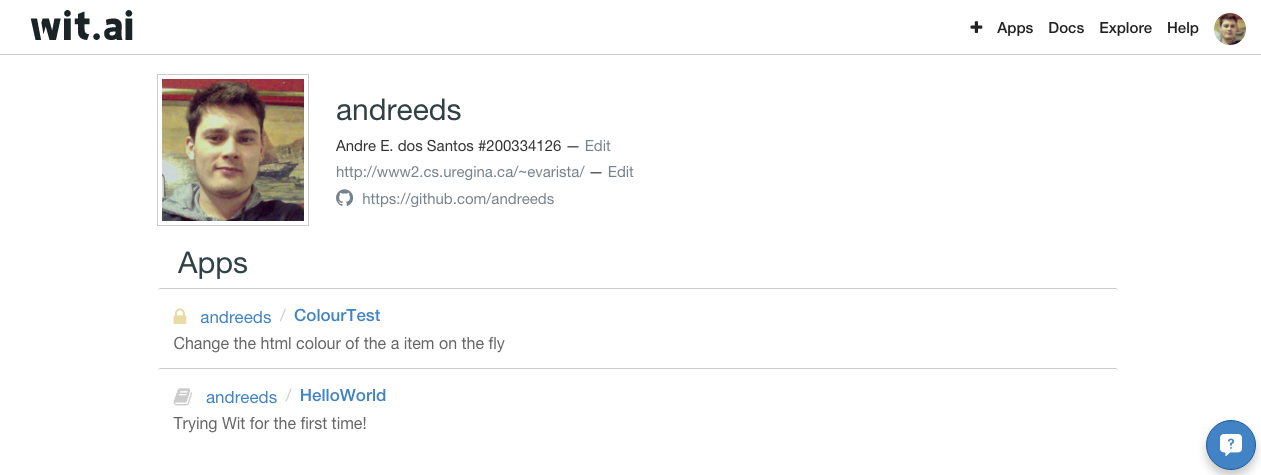
\includegraphics[width=\textwidth]{figures/Wit_Console.png}
}
\caption{The Wit Console.}
\end{figure}

%\subsection{Determining and Creating User Intent}
\emph{Determining and Creating User Intent}

Given that the user has created a new app, it is time to determine the its intents.
An intent is something that the end-user wants to perform.
For example,
``ask about the weather'', 
``set an alarm on their smartwatch'', and 
``say hello to their robot''.
It is common to focus on a finite list of possible intents.
Hence, each intent corresponds to one action in the app.
For our application, the intent is to ``change the colour of the object'' and also``greetings.''

Once with a raw speech or text input, Wit.ai will determine what is the user intent.

For instance, all the following expressions should be mapped to the same intent:
\begin{lstlisting}[language=html]
``Change the colour to blue''
``Colour: blue''
``I want the colour to be blue''
\end{lstlisting}


There are many different ways to express the same intents. 
Thus, it is the job of Wit.ai to map these expressions to actual intents.

The user can browse existing intents from the community of Wit online.
When typing examples for the intents, Wit will suggest these existing intents. 
If one fits the intent, clicking on “GET” gets a copy of the existing intent in the Wit app.
If there not exist an intent that fits, it is necessary to create a new intent.

To create a new intent, the user must type a name for your new intent in the ``Name your intent'' field.
Usually, intent names try to match the app functions or methods. 
At least three expressions, even with synonymous way to say the same command, must be added.
Figure \ref{fig:entents} shows the intents $colour$ and $greeting$ for the ColourTest App.
Some of the expressions for $colour$ are listed in Example \ref{exe:intent}.


\begin{figure*}[!h]
    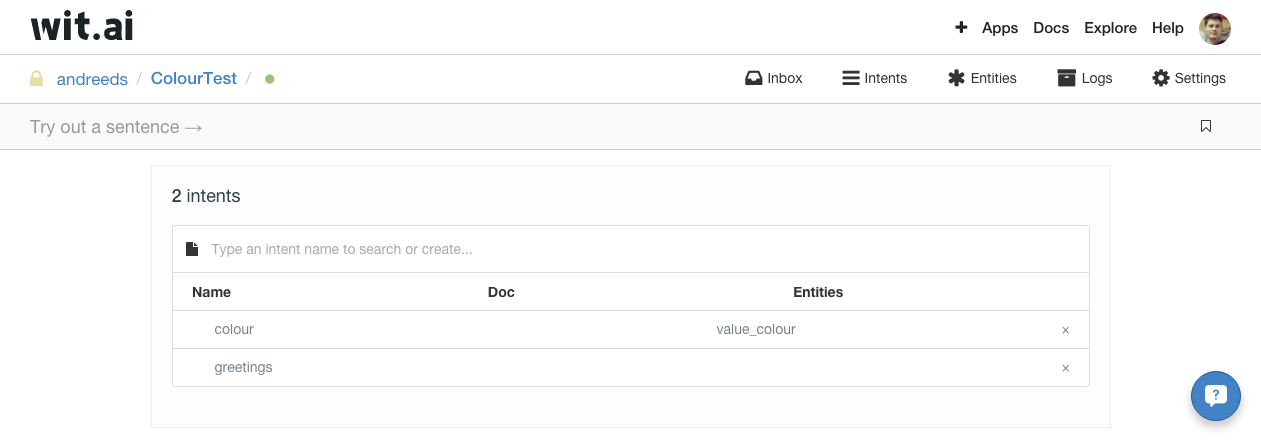
\includegraphics[width=\textwidth]{figures/entities.png}
    \caption{The intents for the ColourTest App.}
    \label{fig:entents}
\end{figure*}


%\subsection{Training}
\emph{Training}

It is time to query the voice app.
At this point, we can already request the voice app via the Wit.ai API.

Notice that, before trainig the app, it is necessary to add the \emph{Client Access Token} to the website.
We will show more details about this step in Section \ref{sec:web}.

In the Inbox of the App we can see the examples said when inputed troght website.

%\subsubsection{Validate Audio from the Inbox}

At Inbox we can validate the the correct sentences recorded by Wit.
Once trained, Wit improves its speech recognitions an the \emph{Confidence} ratio for the expression intents tends to raise.
To train the voice is very simple.
For each expression it reproduces the audio recorded.
If it is correct, we can validate it.
If not, we type the correct sentence and then validate it.

%\subsubsection{Validate Expressions from the Inbox}


At Inbox we can validate matches with expression and intents that were correctly captured by Wit.
For instance, Figure \ref{fig:expressions} shows three expressions captured by Wit, the first one was validated as intent $greetings$, the second was \emph{Archived} since was any of the existing intents, and the third one was validated as intent $colour$.
In our example, we also want to capture the targeted colour.
This is called an \emph{Entity}. 
We can create our own one or select a common one from the dropdown list. 
For instance, the entity $value\_colour$ was created for the intent $colour$, as depicted in Figure \ref{fig:expressions} bottom.


\begin{figure*}[!h]
\begin{center}
    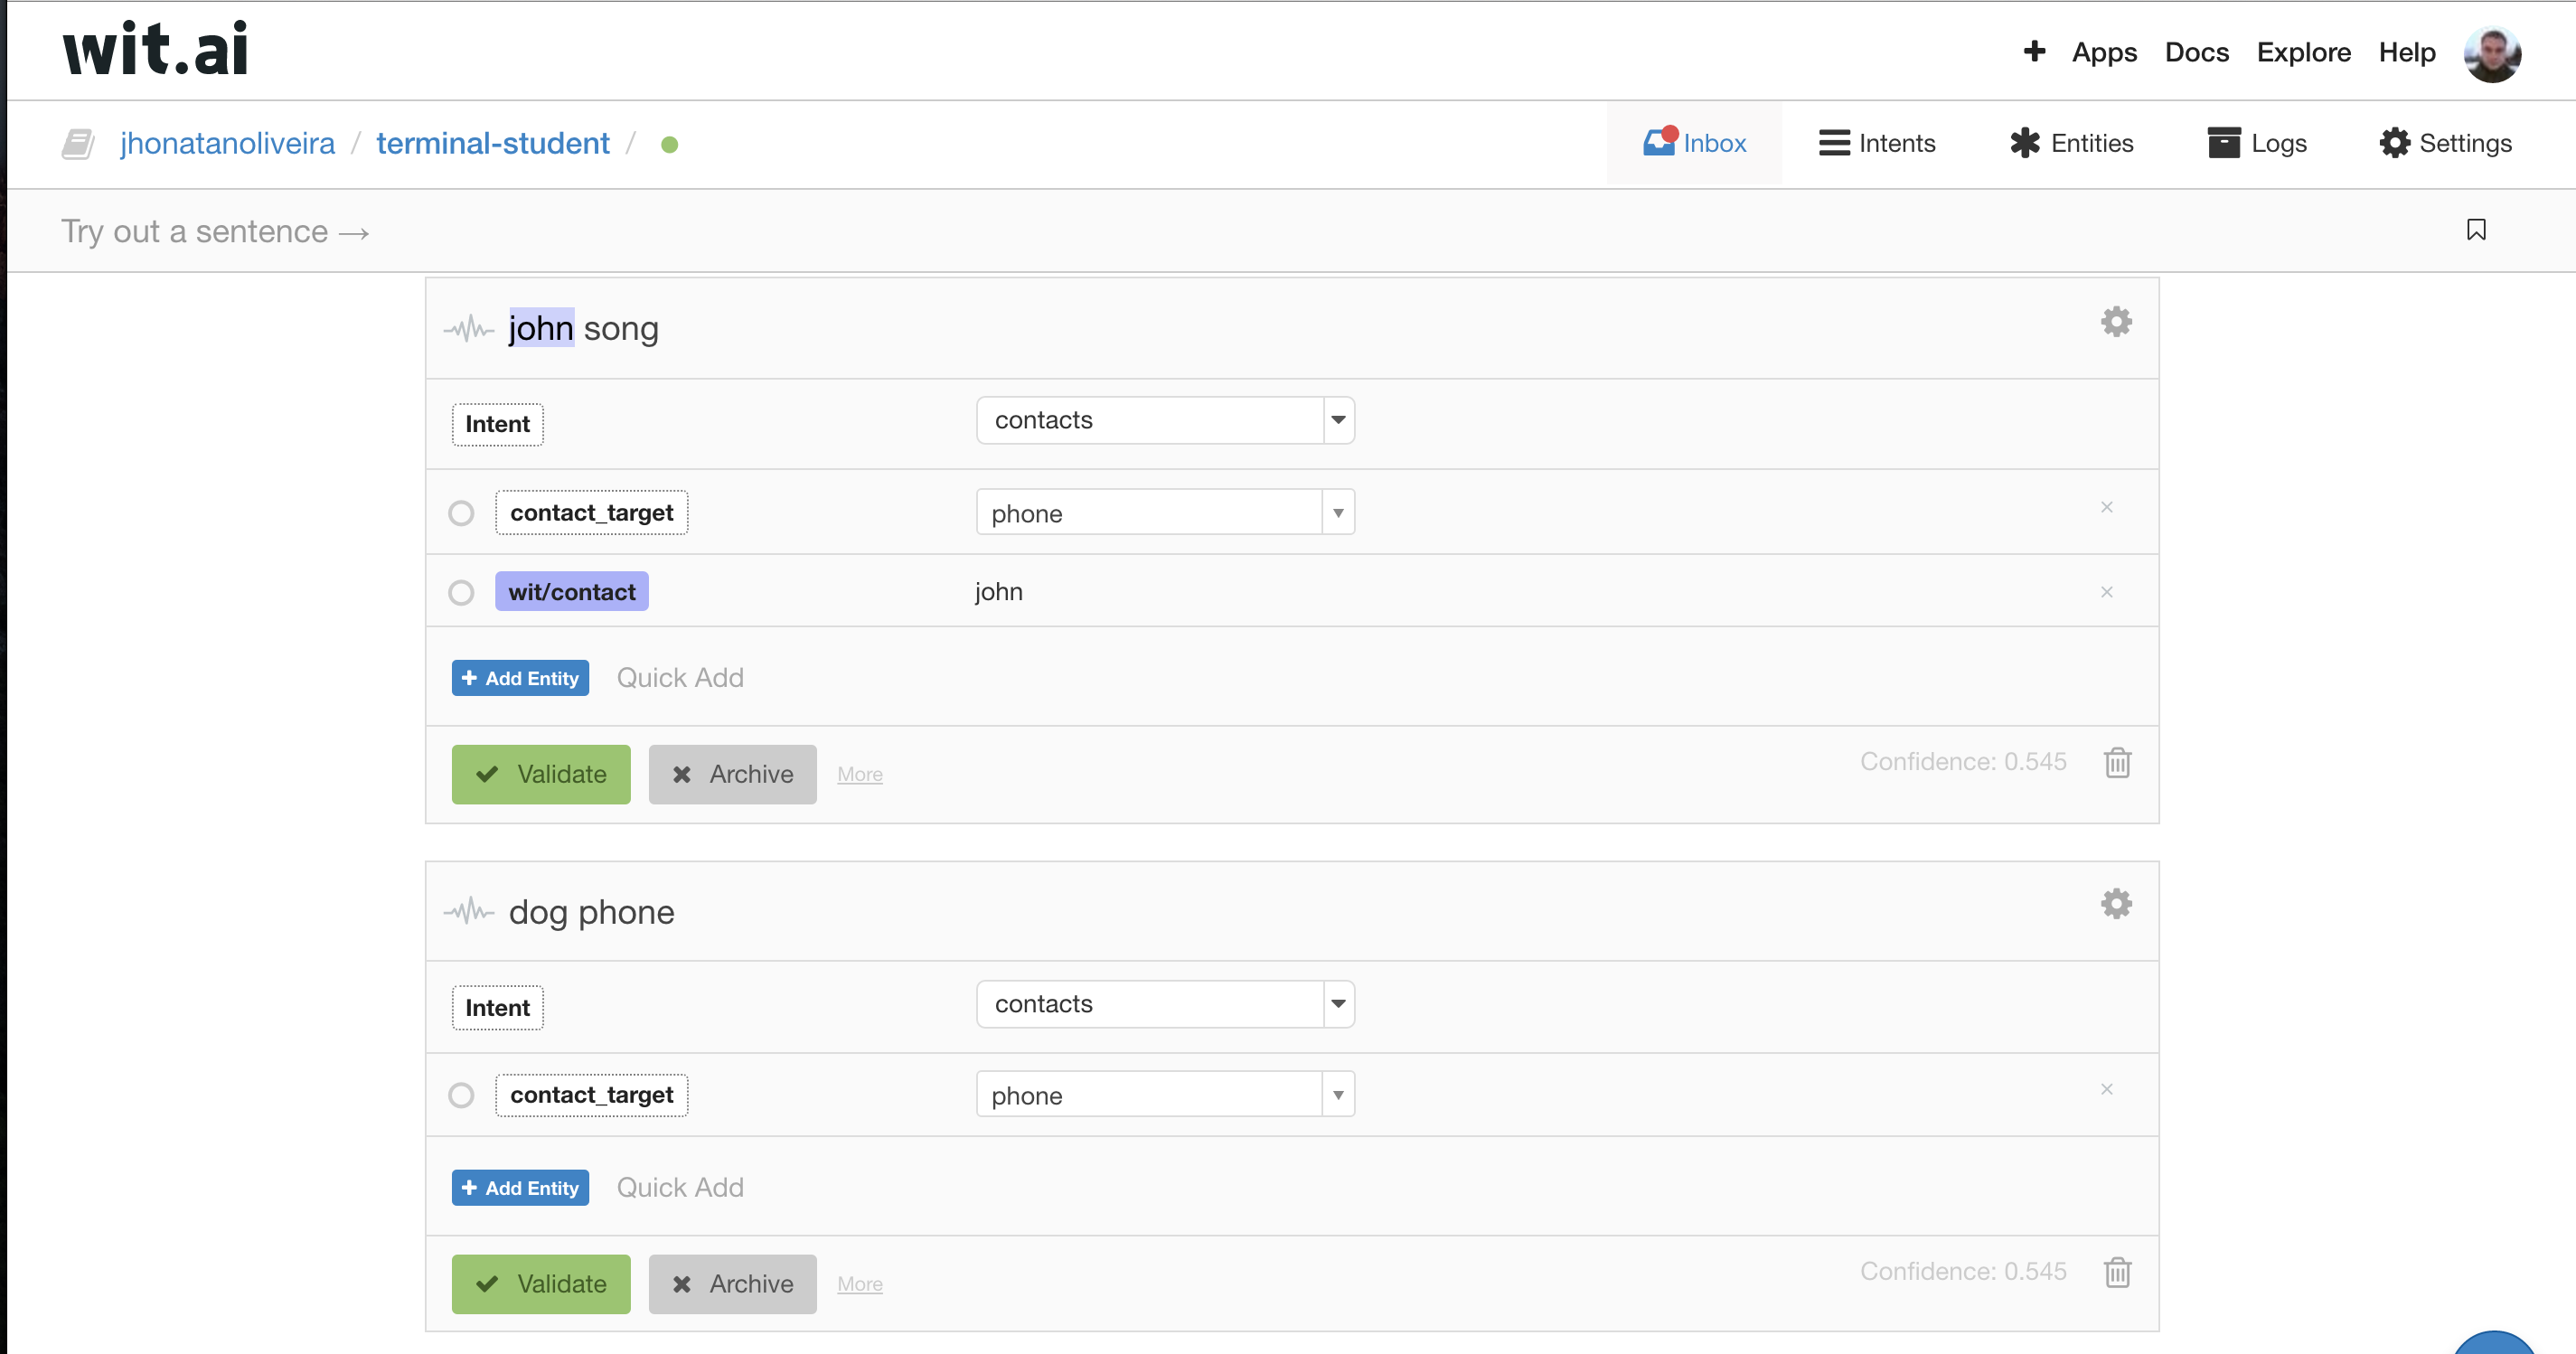
\includegraphics[width=0.75\textwidth]{figures/expressions.png}
    \caption{Expressions captured by Wit.ai.}
    \label{fig:expressions}
\end{center}
\end{figure*}

\subsubsection{Web application}
\label{sec:web}

Now we show how to add Wit to a web app.
As a prerequisites, the browser must support \cite{webrtc}, which is the case of Chrome, Firefox and Opera.

To integrate the voice app with the web app we need to create a new folder for the app, download the \emph{Web SDK} (the microphone app) and extract the archive:
\begin{lstlisting}[language=bash]
	mkdir myapp
	cd myapp
	curl -L <https://github.com/wit-ai/microphone/releases/download/0.7.0/microphone-0.7.0.tar.gz | tar xvzf -
	mv microphone-* microphone
\end{lstlisting}

In the myapp folder, we must create a file $index.html$ containing the html provided by Wit on \url{https://wit.ai/docs/web/0.7.0}.

In the Setting page of the voice app we generate a \emph{Client Access Token}, as illustrated in Figure \ref{fig:token} 
A client access token is unique and authorizes the domain to access the voice app. 
To use the client access token we must replace $CLIENT\_TOKEN$ on the $index.html$ file.
For example, replace 
\begin{lstlisting}[language=java]
	mic.connect("CLIENT_TOKEN");
\end{lstlisting}
for the client access token of our running example, given
\begin{lstlisting}[language=java]
	mic.connect("AWRBY6WLIPAQP7PGCGMQQKKO45LELCWO");
\end{lstlisting}

\begin{figure*}[!h]
\begin{center}
    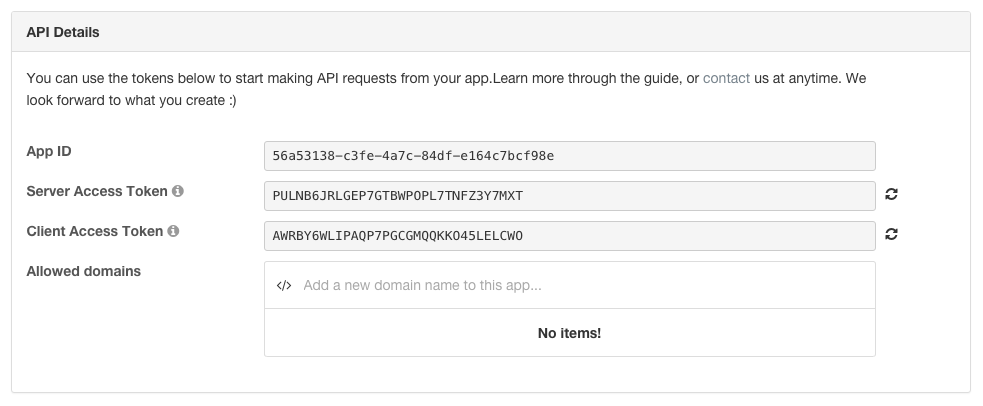
\includegraphics[width=0.75\textwidth]{figures/token.png}
    \caption{A Client Access Token.}
    \label{fig:token}
\end{center}
\end{figure*}


%\subsection{In Action}
\emph{In Action}

To see the web application in action we serve the app with a webserver.
For instance, using Python:
\begin{lstlisting}[language=bash]
	python -m SimpleHTTPServer
\end{lstlisting}
Then, to load the page on the browser
\begin{lstlisting}[language=bash]
	http://localhost:8000
\end{lstlisting}



After allowing your microphone, we will be able to click on the microphone icon and say a command. 
The command will be streamed to the voice app.


\subsubsection{Resource Constrains}



\subsection{Meteor.js}

\emph{Meteor.js} \cite{meteor}, or Meteor for short, is an open-source web platform to create applications using the Web 2.0 paradigmas.
The platform provide a reactive approach by focusing on the data flow.
This is done by creating and managing events in the application.
Also, data management is done with a non-SQL database called \emph{MongoDB} \cite{mongo}.
Meteor simplify the application development by providing an unique programming language, javascript, throughout the whole stack process.
Moreover, the platform makes available a set of common tools for business logic and data management.
Finally, Meteor deploys the application in desktop and mobile without needing to change the source code.

\subsubsection{History and Background}

The Meteor platform was created by a company called Skybreak in 2011 \cite{skybreak}.
Later, in 2012, the company changed its name to Meteor.
The startup was incubated by YCombinator \cite{ycomb} and after receiving an investment of \$11.2 M, the platform development increased considerably.
The platform left beta in October 26th, 2015, with a version that currently provides multiplatform support.

Regarding its internal structure, Meteor is built on top of \emph{Node.js} \cite{node}.
That means that Meteor is driven by events, in order to create an asynchronous model.
This feature is implemented using callback functions: when an event happens a specific function is called to execute a portion of code.
The server-side and client-side are both implemented using javascript.
In the client-side, templates are used to design user interfaces.
Here, a simple markup language defines the design and the events handled by the application.
Meteor has support for more than one template language, being \emph{Blaze} \cite{meteor} the official one.
In the server-side, Meteor handles data management using collections.
The oficial non-SQL database supported is MongoDB, but new ones are being incorporated in future versions \cite{fathom}.


\subsubsection{Getting Started}

Now, we will follow a common flow for an app creation process.
During this section, we will use a single running example which is an application for todo lists.
This todo example can also be found on the official getting started tutorial in \cite{meteor}.
We will try to keep the same code conventions and names always that possible so the reader can use this paper as an extended guide for that tutorial.
We assume that the Meteor program and required 

The following command line is used to create a new application with Meteor:
\begin{lstlisting}[language=bash]
meteor create todo
\end{lstlisting}
This creates a folder structure as shown below:
\begin{lstlisting}[language=bash]
todo.js todo.html todo.css .meteor
\end{lstlisting}
The \emph{todo.js} file is where the javascript code for the server and client stays.
Here is where the code throws and handles events, besides business logic.
Templates for user interface is done in the \emph{todo.html} file with pure HTML markup language and a template markup language.
For this project Blaze is the template languages used.
The \emph{todo.css} file contains styles for the templates.
Lastly, the \emph{.meteor} stores settings and the meteor aplication itself in a hidden folder.

%\subsubsubsection{Templates}
\emph{Templates}

Templates are defined using a special tag called \emph{template}.
Once defined, a template can be included within any HTML code.
In this way, a template is a interface module that can be reuses wherever it is required.
All the HTML code and the templates have access to the data made available in that part of the HTML code.
The basic flow is: the javascript code makes available some data to a specific area of the HTML code (or a specific template), so the template language can access that data and print the ones of interest for the user.
Bellow, we show a simple todo list interface.

\begin{lstlisting}[language=html,escapechar=|]
<head>
  <title>Todo List</title>
</head>
 
<body>
  <div class="container">
    <header>
      <h1>Todo List</h1>
      <form class="new-task">  |\label{code:form_b}|
        <input type="text" name="text" placeholder="Type to add new tasks" />
      </form>  |\label{code:form_e}|
    </header>
 
    <ul>
      {{#each tasks}}
        {{> task}} |\label{code:temp}|
      {{/each}}
    </ul>
  </div>
</body>
 
<template name="task">  |\label{code:temp_b}|
  <li class="{{#if checked}}checked{{/if}}"> |\label{code:checked}|
    <button class="delete">&times;</button>  |\label{code:delete}|
    <input type="checkbox" checked="{{checked}}" class="toggle-checked" />
    <span class="text">{{text}}</span>
  </li>
</template>  |\label{code:temp_e}|
\end{lstlisting}

Here, the HTML code defines in its \emph{body} a title and a list.
Notice that Blaze commands are defined within \emph{\{\{} and \emph{\}\}}.
In the list, the Blaze command \emph{\#each} goes through a list of data, as in a loop lace.
The data variable \emph{tasks} contains this list of data and was made available to this part of the code by the javascript code.
The Blaze command \emph{$>$ name\_of\_template} prints a template previously defined with name \emph{name\_of\_template}.
In lines \ref{code:temp_b}-\ref{code:temp_e}, the template named \emph{task} is defined.
This template expect to find available in its scope a data variable called \emph{text}.
In line \ref{code:temp}, the template is included in that spot of the HTML code and the data variable \emph{text} is available on the loop scope of the \emph{\#each} command.
Note that \emph{text} is a field within \emph{tasks}.

On the javascript file we define code for the client and server.
In order to distinguish between them, Meteors makes available a global variable called \emph{isClient}, which goes to true if the running environment is the browser and goes to false if it is the Node.js one.
If a code is called without being under the conditions of a client or server, the code is run in both environments.
Follows the javascript code to create a simple database where the \emph{tasks} are saved.

\begin{lstlisting}[language=java,escapechar=|]
Tasks = new Mongo.Collection("tasks");  |\label{code:db}|
 
if (Meteor.isClient) {  |\label{code:cond}|

  // This code only runs on the client
  Template.body.helpers({  |\label{code:help_b}|
    tasks: function () {  |\label{code:func}|
      return Tasks.find({});
    }  |\label{code:help_e}|
  });
  
  Template.body.events({
    "submit .new-task": function (event) {  |\label{code:event}|
      // Prevent default browser form submit
      event.preventDefault();
 
      // Get value from form element
      var text = event.target.text.value;
 
      // Insert a task into the collection
      Tasks.insert({
        text: text,
        createdAt: new Date() // current time
      });
 
      // Clear form
      event.target.text.value = "";
    }
  });
  
  Template.task.events({
    "click .toggle-checked": function () {  |\label{code:event_checked}|
      // Set the checked property to the opposite of its current value
      Tasks.update(this._id, {
        $set: {checked: ! this.checked}
      });
    },
    "click .delete": function () {  |\label{code:delete_java}|
      Tasks.remove(this._id);
    }
  });
  
}
\end{lstlisting}

Line \ref{code:db} runs on the server and on the client, since it is not inside the conditional in line \ref{code:cond}.
In the server, that command creates a database called \emph{tasks} if it does not exist already.
In the client, it creates a cache of the same database where Meteor manages some saved data in order to reuse repeated queries from the user.
From line \ref{code:help_b} to \ref{code:help_e}, using the global variable \emph{Template}, we make available to the \emph{body} of the HTML whatever data the not named function in line \ref{code:func} return.
The function returns all the entries in the previously created \emph{tasks} database.
These returned data is available to the HTML code on a data variable called \emph{tasks}, as determined in line \ref{code:func}.

%\subsubsubsection{Inserting Data}
\emph{Inserting Data}

Regarding the data inclusion, this HTML code has a form which will receive the new input data from the user.
Lines \ref{code:form_b}-\ref{code:form_e} defines a simple form where the user can input new tasks.
When pressing enter, an event is thrown from the HTML code and can be handled in the javascript code.

The javascript code watch for an event for the form submission, as shown in line \ref{code:event}.
From here, the default reaction of the browser, which is try to submit the form, is stopped.
The, the value of the input text is saved in a variable.
Next, the cached database variable \emph{Tasks} is used to insert a new entry on the server database with the text saved from the user input.
Finally, the text input is cleared.

Notice in the last insertion process that the cached database was used to update the server database.
This is possible due to the way Meteor works in client and server.
The client has only a cached version of the database.
But whenever this cached version is updated, an event goes to the server (whenever there is connection available) making the server database to update.
The other way around works in the same manner: if the server database is updated, an event goes to all client spreading the update.

%\subsubsubsection{Updating and Removing Data}
\emph{Updating and Removing Data}

If a task is done, we want to check it out from the list by updating its entry with a done flag.
In the HTML code, line \ref{code:checked}, the template \emph{task} has a conditional statement checking for a variable called \emph{checked}.
If the variable is true, the body of the condition, which is just a string \emph{checked}, is executed.
This variable, as expected, is set in the javascript code.
Indeed, in line \ref{code:event_checked}, the javascript watch for an event of a click on the checkbox.
If it happens, the cached database \emph{Tasks} is updated by setting a field \emph{checked} to the opposite value that the user entered.
Notice the use of a special variable \emph{this} which provides context for HTML access from where the event occurred.


The deletion process is similar to updating but a different function is used on the cached database.
The javascript code, line \ref{code:delete}, watch for the HTML code, line \ref{code:delete}.
When the user clicks in the delete button, the javascript code is executed by removing the correspondent id of the entry.
Again, note the use of \emph{this} as a context variable for the entry where the event occurred.

\subsubsection{Resource Constrains}

Meteor can be used to build resource constrain products.
In this type of application, the amount of processing and memory are often restricted.
Therefore, the use of parallel computing or decentralized tasks are common and necessary.
Meteor can be use to avoid heavy load computation in the limited hardware itself.
A server can be used to process all the required heavy workload while the client simply show in real time the results.

One way of providing an interface to a Meteor server side is by using the official server-client protocol, called \emph{Distributed Data Protocol} (DDP).
The DDP protocol is a simple specification on how other languages can communicate with a Meteor server.


\subsection{Raspberry Pi}

%todo add photo resppi
The \emph{Raspberry Pi} a low cost is single-board computer developed in the UK by the Raspberry Pi Foundation with the intention of stimulating the teaching of basic computer science in schools \cite{pi2012raspberry}.
It is a capable small device that is capable of doing everything a desktop computer does, from browsing the internet and playing high-definition video, to making spreadsheets, word-processing, and playing games \cite{resp2}.

The Raspberry Pi has a Broadcom BCM2835 system on a chip (SoC), which includes an ARM1176JZF-S 700 MHz processor, VideoCore IV GPU, and 256 megabytes of RAM. 
It uses an SD card for booting and long-term storage.
The Raspberry Pi 2 Model B is the second generation Raspberry Pi. 
It replaced the original Raspberry Pi 1 Model B+ in February 2015. 
Compared to the Raspberry Pi 1 it has: (i) A 900MHz quad-core ARM Cortex-A7 CPU and (ii) 1GB RAM \cite{resp2}.



\subsubsection{History and Background}

%todo adjust
In 2006, early concepts of the Raspberry Pi were based on the Atmel ATmega644 microcontroller \cite{wong2011build}.
The Model A was not the first Raspberry Pi to hit general availability – that distinction went to the Model B. 
The A was, nevertheless, the truest to the bare-bones ethos of the Pi project, retailing for \$25 and initially packing just 128MB of memory. (Later raised to 256MB.)

\subsubsection{Getting Started}

Required:
SD Card. The newer Raspberry Pi Model A+, Raspberry Pi Model B+, Raspberry Pi 2 Model B, Raspberry Pi Zero, and Raspberry Pi 3 Model B require micro SD cards.
Display and connectivity cables
Keyboard and mouse
Power supply

Not essential but helpful to have

    Internet connection
        To update or download software, we recommend that you connect your Raspberry Pi to the internet, either via an Ethernet cable or a WiFi adapter.


Plugging in your Raspberry Pi

Before you plug anything into your Raspberry Pi, make sure that you have all the equipment listed above to hand. Then follow these instructions:

    Begin by slotting your SD card into the SD card slot on the Raspberry Pi, which will only fit one way.
    Next, plug your USB keyboard and mouse into the USB slots on the Raspberry Pi.
    Make sure that your monitor or TV is turned on, and that you have selected the right input (e.g. HDMI 1, DVI, etc.).
    Then connect your HDMI cable from your Raspberry Pi to your monitor or TV.
    If you intend to connect your Raspberry Pi to the internet, plug an Ethernet cable into the Ethernet port next to the USB ports, otherwise skip this step.
    When you are happy that you have plugged in all the required cables and SD card, plug in the micro USB power supply. This action will turn on and boot your Raspberry Pi.
    If this is the first time your Raspberry Pi and NOOBS SD card have been used, then you will have to select an operating system and configure it. Follow the NOOBS guide to do this.

Read more in our documentation.

\subsubsection{Resource Constrains}

The main disadvantages of Raspberry Pi are \cite{vujovic2014raspberry}:

It does not have a real-time clock (RTC) with a backup battery but it can easily work around the missing clock using a network time server, and most operating systems do this automatically.

It does not have a Basic Input Output System (BIOS) so it always boots from an SD card.

It does not support Bluetooth or WiFi out of the box but these supports can be added by USB dongles.

Unfortunately, most Linux distributions are still a bit
picky about their hardware, so it should be first checked whether flavor of Linux supports particular device.

It doesn’t have builtin an Analog to Digital converter. External component must be used for AD conversion.

It has a relatively small number of digital I/O, but it can be expanded with external logic devices.

\section{Implementation}

%- Administration scheme:
%    - Services
%        - Data
%            - Knowledge tree
%                - The tree is built in server not in client
%        - External
%            - Map with key-value being the key the name of the external service and the value a function which runs the service
%- Searching the tree
%    - scoring the tree with one pass
%    - problem: when we have the query found in the parent and child. Eg: tainara -> tainara@gmail.com


How the project works.

- Administration scheme:
    - Services
        - Data
            - Knowledge tree
                - The tree is built in server not in client
        - External
            - Map with key-value being the key the name of the external service and the value a function which runs the service

- Searching the tree
    - scoring the tree with one pass
    - problem: when we have the query found in the parent and child. Eg: tainara -> tainara@gmail.com

% add as section:  Description of design process
\subsection{Description of design process}
Design process.

%add as section:Discussion of group contributions
\subsection{Discussion of group contributions}



\section{Results}

Failures and successes.


 % INCLUDE: the project
\chapter{The Ex-Project}
\label{sec:ex-project}

\cleanchapterquote{TODO.}{TODO}{(TODO)}

The initial plan for our final project included a service inside the app for indoor navigation.
The idea was to allow the user to ask for a location within the University of Regina main campus and the app would trace a route from where the device hosting the app is to where the user requested.
Indoor navigation itself is a complex and well known task problem in computer science and engineering.
Our primary focus was to use some already available solution for indoor navigation, instead of trying to come up with our own solution.
In this way, we wanted to show how resource constrain devices can still be used to provide such service by using cloud computing.

We did a broad research on publicly available solutions for indoor navigation, including paid, free or open source ones.

\begin{figure}
\label{fig:console}
\centerline{
\includegraphics[width=\textwidth]{figures/chip_gps.png}
}
\caption{}
\end{figure} % INCLUDE: the ex project
\chapter{Conclusion}
\label{sec:conclusion}

\cleanchapterquote{TODO.}{TODO}{(TODO)}
 % INCLUDE: conclusion

\cleardoublepage

% --------------------------
% Back matter
% --------------------------
%{%
%\setstretch{1.1}
%\renewcommand{\bibfont}{\normalfont\small}
%\setlength{\biblabelsep}{0pt}
%\setlength{\bibitemsep}{0.5\baselineskip plus 0.5\baselineskip}
%\printbibliography[nottype=online]
%\printbibliography[heading=subbibliography,title={Webseiten},type=online,prefixnumbers={@}]
%}
%\cleardoublepage
%
%\listoffigures
%\cleardoublepage
%
%\listoftables
%\cleardoublepage

\bibliographystyle{splncs03}
\bibliography{references}

%% !TEX root = ../thesis-example.tex
%
\pagestyle{empty}
\hfill
\vfill
\pdfbookmark[0]{Colophon}{Colophon}
\section*{Colophon}

This thesis was typeset with \LaTeXe.
It uses the \textit{Clean Thesis} style developed by Ricardo Langner.
The design of the \textit{Clean Thesis} style is inspired by user guide documents from Apple Inc.

Download the \textit{Clean Thesis} style at \url{http://cleanthesis.der-ric.de/}.

%\cleardoublepage
%test

%% !TEX root = ../thesis-example.tex
%
%************************************************
% Declaration
%************************************************
\pdfbookmark[0]{Declaration}{Declaration}
\chapter*{Declaration}
\label{sec:declaration}
\thispagestyle{empty}

You can put your declaration here, to declare that you have completed your work solely and only with the help of the references you mentioned.

\bigskip

\noindent\textit{\thesisUniversityCity, \thesisDate}

\smallskip

\begin{flushright}
	\begin{minipage}{5cm}
		\rule{\textwidth}{1pt}
		\centering\thesisName
	\end{minipage}
\end{flushright}

%*****************************************
%*****************************************

%\clearpage

%\newpage
%\mbox{}

% **************************************************
% End of Document CONTENT
% **************************************************
\end{document}
